\documentclass{article}
\usepackage[utf8]{inputenc}
\usepackage[spanish]{babel}
\usepackage{graphicx}
\usepackage{anysize}
\usepackage{fancyhdr} 
\usepackage[export]{adjustbox}
\usepackage{titlesec}
\usepackage{enumitem}
\usepackage{listings}
\usepackage{xcolor}
\usepackage{array}
\usepackage{longtable}
\usepackage{multicol}
% \usepackage{hyperref}
% \usepackage{float}
% \usepackage{tabu}
\usepackage{subcaption}

% Izquierda, derecha, arriba, abajo
\marginsize{2cm}{2cm}{1.2cm}{1.5cm} 
\renewcommand{\familydefault}{\sfdefault}
\decimalpoint%

\graphicspath{{assets/}{tema04-ej-prac-02.assets/}}

\setlength{\parindent}{0in}
\titleformat*{\section}{\large\bfseries}

% Para insert código
\definecolor{codegreen}{rgb}{0,0.6,0}
\definecolor{codegray}{rgb}{0.5,0.5,0.5}
\definecolor{codepurple}{rgb}{0.58,0,0.82}
\definecolor{backcolour}{rgb}{1,1,1}

\usepackage{textcomp}
\lstset{upquote=true}
\lstdefinestyle{mystyle}{
    backgroundcolor=\color{backcolour},   
    commentstyle=\color{codegreen},
    keywordstyle=\color{magenta},
    numberstyle=\tiny\color{codegray},
    stringstyle=\color{codepurple},
    basicstyle=\ttfamily\footnotesize,
    breakatwhitespace=false,         
    breaklines=true,                 
    captionpos=b,                    
    keepspaces=true,                 
    % numbers=left,                    
    % numbersep=5pt,                  
    showspaces=false,                
    showstringspaces=false,
    showtabs=false,                  
    tabsize=2
}

\lstset{style=mystyle}

\newcommand{\materia}{BDA}
\newcommand{\clave}{2929}
\newcommand{\profesor}{Ing. Rodriguez Campos \textsc{Jorge Alberto}}
\newcommand{\grupo}{1}
\newcommand{\semestre}{2021-1}

\newcommand{\alumno}{Francisco Pablo \textsc{Rodrigo}}

\newcommand{\actividad}{Tema 04 \\ Ejercicio práctico 02}
\newcommand{\titulo}{Administración de las estructuras de Memoria}

\newcommand{\fechaEntrega}{16 de diciembre de 2020}

%%%%%%%%%%%%%%%%%%%% ENCABEZADO %%%%%%%%%%%%%%%%%%%%%%%%%%%%
\pagestyle{fancy}
\fancyhf{}
\renewcommand{\headrulewidth}{0pt}
\fancyhead[R]{% Left header
    {\renewcommand*{\arraystretch}{1}
    \begin{tabular}{l}
        \materia \\ 
        \actividad%
    \end{tabular}}
    \,% Space
    \rule[-1.75\baselineskip]{0pt}{0pt}
    % Strut to ensure a 1/4 \baselineskip between image and header rule
    
\includegraphics[height=3\baselineskip,valign=c]{unam}
}
\setlength{\headsep}{0.3in}


\begin{document}
%%%%%%%%%%%%%%%%%%% DATOS PORTADA %%%%%%%%%%%%%%%%%%%%%%%%
\thispagestyle{empty}
\begin{minipage}[t][5cm][t]{0.2\linewidth}
    
\includegraphics[width=2.5cm]{unam.jpg}
    \vspace{10cm}

    
\includegraphics[width=2.5cm]{fiblack}
\end{minipage}
\begin{minipage}[t]{0.7\linewidth}
    \vspace{-2.5cm}
    \LARGE{\textbf{Universidad Nacional Autónoma de México}}\\
    \Large{\textbf{Facultad de Ingeniería}} \\

    \large{\semestre}\\[2cm]

    \large{\textbf{\materia (\clave)}}\\
    \large{\textbf{Gpo: 1}}\\[5mm]
    \large{\textbf{Profesor:} \profesor}\\ [1.5cm]
    \begin{center}
        \LARGE{\textbf{\actividad}}\\
        \LARGE{\textbf{\titulo}}\\
    \end{center}

    \vspace{3.3cm}

    \large{\textbf{Alumno:} \alumno} \\[1.5cm]

    \begin{flushright}
        \fechaEntrega%
    \end{flushright}
\end{minipage}

\newpage
%%%%%%%%%%%%%%%%%%% CONTENIDO %%%%%%%%%%%%%%%%%%%%%%%%

\section*{Objetivos}

Comprender y revisar las principales vistas del diccionario de datos que 
muestran información acerca de la cantidad de memoria que se le asigna
al db buffer cache, en particular al default pool. A partir de una serie de 
actividades, comprender y analizar la forma en la que se leen buffers en del
default pool: lecturas físicas (de los data files), lecturas del caché y 
lecturas consistentes.
Comprender y configurar JMeter como herramienta principal
para simular operaciones simultáneas realizadas por diversos usuarios.


\section*{C1. Código DDL y resultado al consultar la tabla
\texttt{t03\_db\_buffer\_cache}}

\lstinputlisting[language=SQL,firstline=38,lastline=48]
  {tema04-ej-prac-02-codigo/s-01-crea-objetos.sql}

  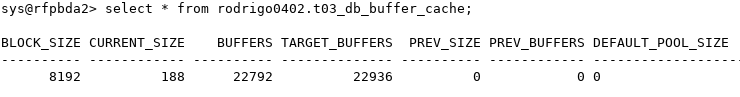
\includegraphics[width=0.9\linewidth]{c1}

  \begin{itemize}
    \item \textbf{Respuesta pregunta A. Implicaciones valores en cero para
      \texttt{current\_size, target\_size, target\_buffers}} \\[3mm]
      Como la base de datos esta recién iniciada y no ha habido operaciones 
      de ningún tipo (DML o DQL) no ha sido necesario utilizar los buffers y por 
      lo tanto los parámetros estarán en cero.

    \item \textbf{Respuesta pregunta B. Implicaciones valores en cero para
      \texttt{prev\_size y pref\_buffers}}\\[3mm]
      Indican que para la última operación realizada los valores fueron cero,
      es decir no se han realizado operaciones.

    \item \textbf{Respuesta pregunta C. Implicaciones valores en cero para
      \texttt{default\_pool\_size}}\\[3mm]
      Indica que no se han realizado escrituras o lecturas.
      
  \end{itemize}

\section*{C2. Código DDL y resultado al consultar la tabla
  \texttt{t04\_db\_buffer\_sysstats}}

\lstinputlisting[language=SQL,firstline=49,lastline=80]
  {tema04-ej-prac-02-codigo/s-01-crea-objetos.sql}

  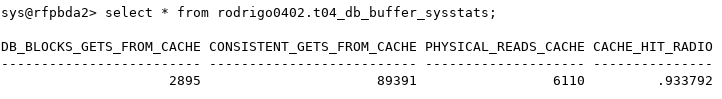
\includegraphics[width=0.9\linewidth]{c2}

  \begin{itemize}
    \item \textbf{Respuesta pregunta A. Valores de \texttt{cache\_hit\_radio}
      que indican una correcta cantidad de memoria para el default pool.\\
      ¿Qué valores debería tener \texttt{cache\_hit\_radio} para considerar 
      que el db buffer cache está correctamente configurado, es decir, las 
      lecturas físicas se minimizan?} \\[2mm]
    
      El valor debe estar entre 0.9 y 0.95 (intervalo abierto)

    \item \textbf{Respuesta pregunta B. Valores de \texttt{cache\_hit\_radio}
      que indican una cantidad incorrecta de memoria para el default pool.\\
      ¿Qué valores debería tener \texttt{cache\_hit\_radio} para considerar 
      que el db buffer cache requiere un aumento de memoria debido a un 
      incremento de lecturas físicas.}\\[2mm]

      El valor ronda entre 0.95 y 1

  \end{itemize}

\section*{C3. Pantalla JMeter}

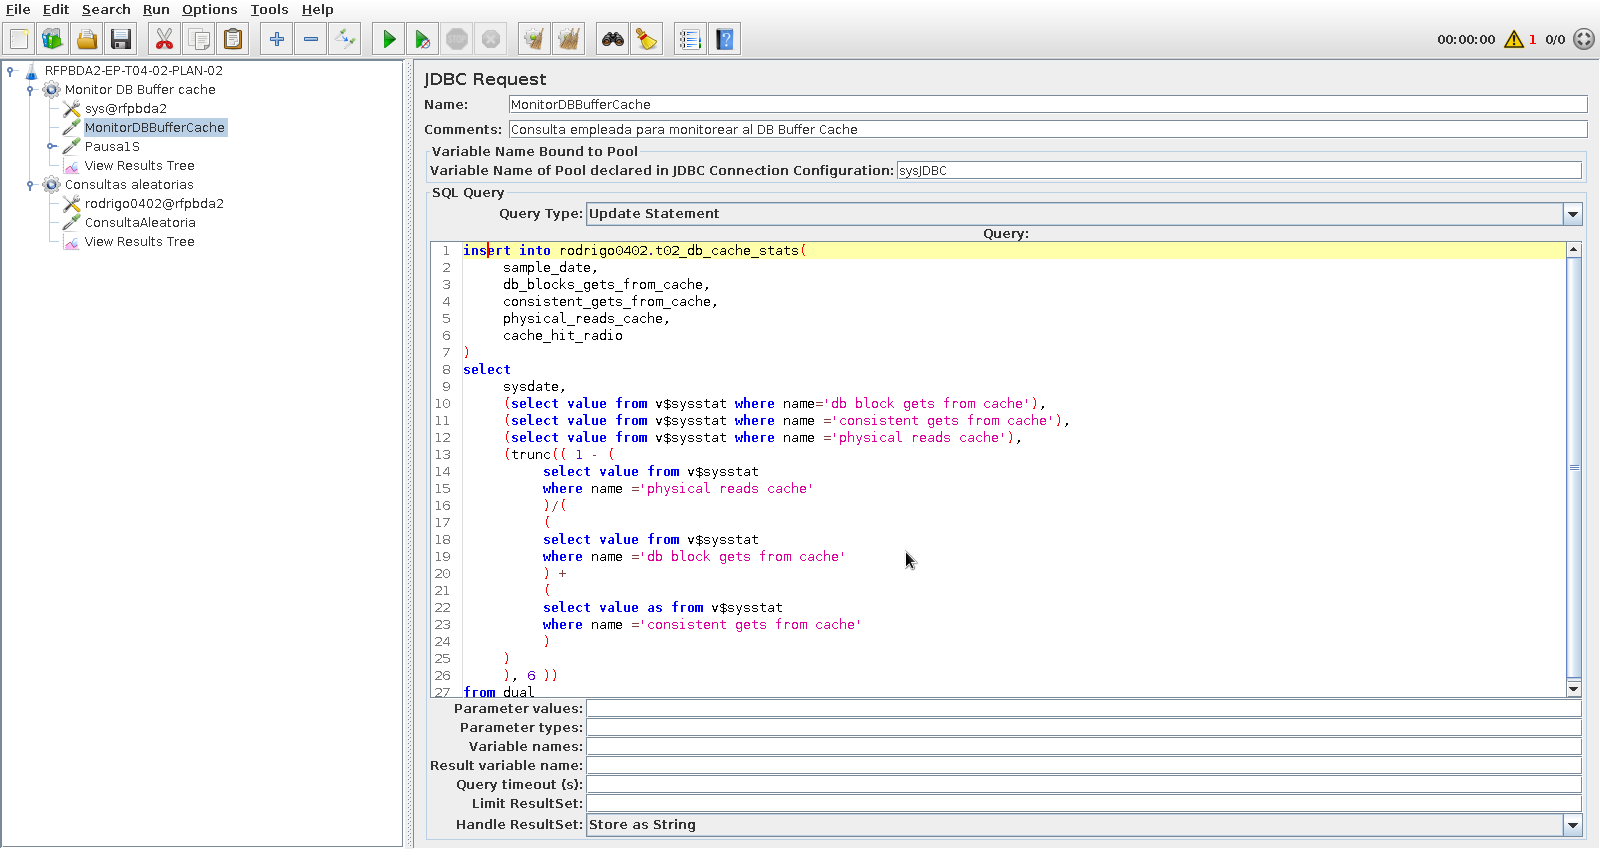
\includegraphics[width=\linewidth]{jmeter}

\newpage

\section*{C4. Gráficas y análisis de resultados}

\begin{figure}[ht!]
  \begin{subfigure}{0.5\textwidth}
    \centering  
    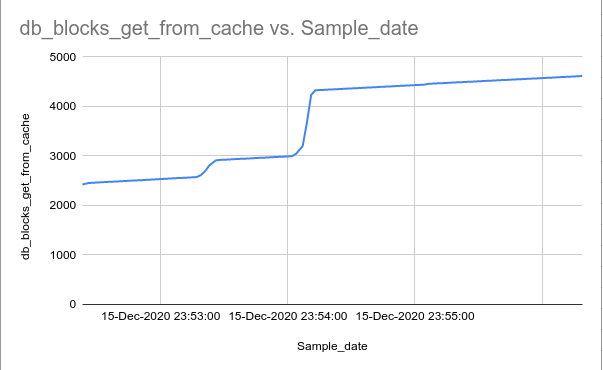
\includegraphics[width=0.9\linewidth]{grafica01}
    \caption{}
  \end{subfigure} 
  \begin{subfigure}{0.5\textwidth}
    \centering  
    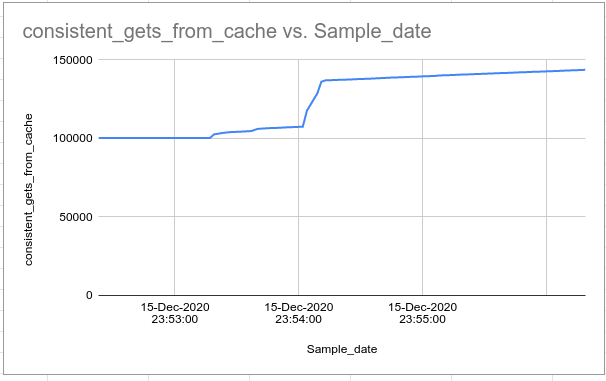
\includegraphics[width=0.9\linewidth]{grafica02}
    \caption{}
  \end{subfigure} 
  \newline
  \\[3mm]
  \begin{subfigure}{0.5\textwidth}
    \centering  
    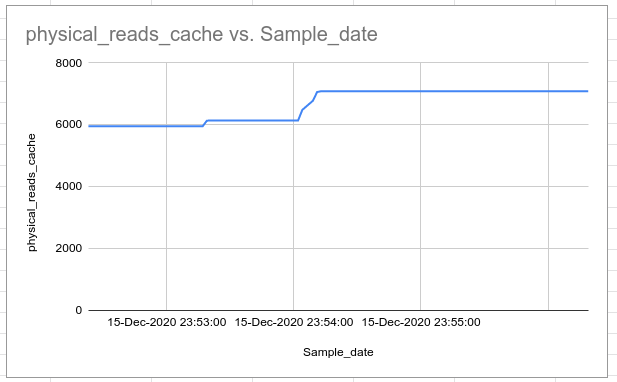
\includegraphics[width=0.9\linewidth]{grafica03}
    \caption{}
  \end{subfigure} 
  \begin{subfigure}{0.5\textwidth}
    \centering  
    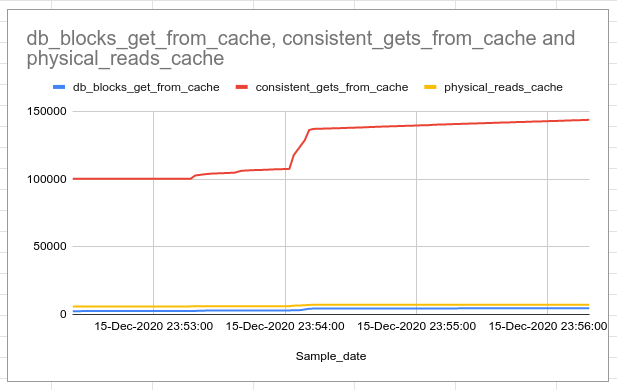
\includegraphics[width=0.9\linewidth]{grafica04}
    \caption{}
  \end{subfigure} 
\end{figure}

En las gráficas (a) y (b) se puede ver que en el primer minuto el tamaño de los
bloques de memoria (RAM) leídos permanece casi constante. Posteriormente, el
tamaño de bloques empieza a incrementar y esto se debe a que se empieza a
ejecutar la consulta del segundo hilo de Jmeter. De hecho tanto en la gráfica
(a) como en la gráfica (b) se ve ese punto de quiebre en el cual el tamaño de 
dicho buffers aumenta. De estas gráficas es interesante notar que no 
el tamaño de buffers aumenta drásticamente por un tiempo pero después deja de
crecer tan rápidamente, esto debido a que cada vez más datos se encuentran en
memoria y no es necesario incrementar el tamaño del buffer utilizado.\\

Ahora bien, si analizamos la gráfica (c), que corresponde las lecturas físicas,
en nuestro caso a disco, observaremos que pasa algo similar que en (a) y (b).
En el primer minuto las lecturas son prácticamente constantes y después
tiene un punto de quiebre que nos indica que se están empezando a realizar 
consultas de nuestros datos. Sin embargo, después de un tiempo se estabiliza 
porque los datos se encuentran ya en memoria y no es necesario leer más bloques
del disco.\\

Finalmente, para la gráfica (d), podemos ver la comparación entre las lecturas
a disco y las lecturas al buffer. Se observa que las lecturas a disco son 
mucho mayores que las lecturas a los buffers. Lo anterior es importante porque
nos permitirá hacer el afinamiento de la base de datos con el fin de reducir
las lecturas a disco.

\section*{C5. Resultado del validador}

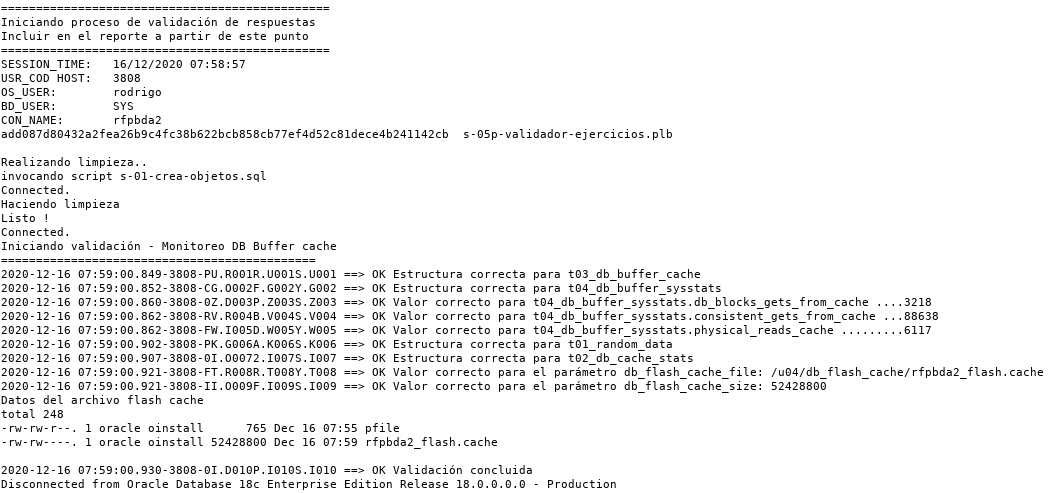
\includegraphics[width=\linewidth]{validador}

\section*{Comentarios y conclusiones}

En esta práctica tuvimos un primer acercamiento a lo que podría ser una base
de datos productiva, como comentario puedo decir que es muchísimo muy diferente
al ambiente local en donde se realizan consultas en modo monousuario y todo
sale bien y no hay carga de trabajo, sin embargo al incluir múltiples usuario
se observa de manera tangible el estresamiento de los equipos personales, en 
el caso de mi computadora en ventilador empezó a girar más rápido y el equipo
se notó ligerarmente más caliente y esto no es nada si lo comparamos un 
servidor que tiene que estar atentiendo a múltiples usuarios las 24 hrs. del 
día. \\

Por otra parte, gracias a los ejercicios propuestos se pudo analizar la 
importancia de tener una base de datos bien configurada ya que de los contrario
las múltiples lecturas a disco nos afectarán en desempeño.

\renewcommand\refname{Bibliografía y referencias}
\begin{thebibliography}{99}
    \bibitem{burleson} Burleson Consulting. \textit{Oracle tips } en 
    \texttt{http://www.dba-oracle.com/oracle\_news/}
  \bibitem{oracle} Oracle Help Center. \textit{Database Performance Tuning 
    Guide} en \texttt{https://docs.oracle.com/database/\\%
    121/TGDBA/tune\_buffer\_cache.htm\#TGDBA294}
\end{thebibliography}

\end{document}
\section*{Comentarios y conclusiones}
